\subsection{Tool development}
\label{ssec:toolDev}
This tool is divided into two scripts, one for Linux and another for Windows, allowing them to execute native system commands and thus making them more adapted to their environment and limitations. 

Given that the two scripts use the same structure, the first step in this development was both a definition of the main flow of the program and the creation of a general design, to organize how the final code would be divided. After that, both scripts have been coded, combining implementation phases with short testing phases, to check that each function worked as it should. 

\subsubsection{Scripts research and analysis}
But before starting with the design, and after learning about other tools with similar functions, as seen in the \textit{Research} section, the code of some of that tools was analysed in order to study what features were desirable in a tool of this type, and how to implement some of them if possible, to speed up the following tasks.

A \textit{script} is usually a "small" piece of code (a single file with a few thousand lines of code), written in an interpreted language that has direct access to operating system functions, used to automate the execution of tasks\cite{WikiScript}. Some examples of programming languages used for scripting are \texttt{bash} or Python for Linux, as they are installed by default in most Linux distributions, and \texttt{cmd}, Visual Basic Application (\texttt{.vba}) or PowerShell for Windows, as they are system native.

The general characteristics of a script are:
\begin{itemize}
\item Simple syntax and semantics: lack of classes or functions, use of global variables,...
\item Lack of an entry point, the code is executed from start to finish
\end{itemize}

For this reason, scripts are usually fast to code, but difficult to maintain without proper documentation.

The tools studied in this section were SharPersist\cite{SharPersist}, Linper\cite{Linper} and PowerSploit\cite{PowerView}, explained in sections \ref{sssec:windowsTools}, \ref{sssec:linuxTools} and \ref{sssec:adDisc} respectively. 

\begin{itemize}
\item \href{https://github.com/montysecurity/linper/blob/main/linper.sh}{\textit{Linper}} is a script written in \texttt{bash}, and has the general characteristics above mentioned. It uses some global variables and executes several commands, before creating some functions, that are executed in a final main function. It also provides some usage examples, and some arguments can be given when started to be used during execution time.
%This script uses Python to open TCP connections (using sockets), and modifies the crontab, terminal configuration files and system files (files in "\texttt{/etc}" to implement persistence. It also deploys techniques from other tactics that are not persistence like the cleanup or the "stealth" mode, which are from the \textit{Defense Evasion} tactic.

\item \href{https://github.com/mandiant/SharPersist/blob/master/SharPersist/SharPersist.cs}{\textit{SharPersist}} is a tool written in C\#, which is a semi-compiled language 
%like Java,
developed by Microsoft. This is not a scripting language, so it does not have the typical structure, but it can access the Windows API, so it can use native system functions.
It needs the user to provide arguments too.
% like Linper.
%, and their techniques implementation, even though it is not the same language, are similar to the commands described in the research section, section \ref{sssec:windowsTec}.

\item Finally, the file \textit{Persistence.psm1} of the \href{https://github.com/EmpireProject/Empire/blob/master/data/module_source/persistence/Persistence.psm1}{\textit{PowerSploit}} framework, created by "PowerShellMafia", is a PowerShell module:
%script that is part of a big collection of PowerShell modules, which are 
collections of functions meant to be used, for example, in other scripts, and therefore not having the usual characteristics of a simple script.\\
The \textit{Persistence.psm1} module, though, has lots of documentation on each function, using keywords like ".DESCRIPTION" or ".EXAMPLE" easy reading. These keywords could prove useful when trying to modify or maintain a script because they give extra information.
\end{itemize}

So, the conclusions about the studied tools were that:
\begin{itemize}
\item Some information might need to be provided at execution time, to be able to configure the tool.
\item System native languages are often preferred because of their benefits (having fewer dependencies).
\item It is better to write proper documentation inside the script, to ease its future manipulation.
\end{itemize}

\subsubsection{Design and main functionalities}
\label{ssec:devDesign}
This subsection covers both the analysis and the design phases,
% of the development
 following the waterfall model.

\paragraph{Core design}
When security analysts use a third-party script to perform attacks, it is common to previously modify the used script to customize it to their needs and/or environment variables. 

For that reason, to create this tool design it was necessary to define which main parts would have and how these different parts would be separated, to simplify its understanding and later modification.

As seen in the last section, most of the already created tools used arguments provided by the user in order to launch different techniques; yet, as this tool was meant to be not only automatic but also very configurable, it was determined that using a configuration file instead of arguments would make the tool more accessible to users.
%, so users that do not need to perform very sophisticated deployments can simply modify the given configuration file to be able to use the tool quickly and effortlessly. . 

\pagebreak
With all of that in mind, it was concluded that each script of the developed tool would have the following different components:
\begin{itemize}
\item An \textit{external configuration file}, 
%with different sections as well to simplify its understanding and modification,
which would have the necessary information to run the tool.
\item Lots of different techniques in each script, some similar in both scripts like the \textit{discovery techniques}, and others more adapted to each operating system, like \textit{persistence and backdoor techniques}, all called from a \textit{main function} which would have the program's logic.\\ 
These techniques would be documented and divided using comments, for easy understanding and navigation through the script.
%not to make an assessment of the computer before launching any other technique, and that would be similar for all scripts.
%\item Different, including some that required privileges, that would be executed depending on the information obtained by the discovery techniques. This functions would be adapted to each operating system.
%\item And finally, a \textit{main function} was required to apply all the logic of the program
\end{itemize}

%Also, comments and documentation on the same script are desirable to easy understand and navigate through the script and its functions. And although each language has its own code of documenting, it was determined that some common comments would be used when coding this project's scripts.

These premises were the base to establish the main functionalities of the tool, which defined the different parts that both scripts would be composed.

\paragraph{Program flow}

After some iterations in which functions were tested and discarded, or changed in the flow position, it was concluded that the tool must perform the following steps, adapted to each environment:
\begin{enumerate}
\item Read the configuration file.
\item If an HTTPS backdoor is going to be deployed, search for proxy configurations.
\item Then, check the needed Internet connections (HTTPS, DNS, or ICMP, depending on the configuration file), using the proxy configurations found, if there are any.
\item After that, check if the process where it is running, or the user running it, is privileged.
\item With all the collected evidence, deploy only the available and suitable persistence (which means that, for example, it would not run an HTTPS backdoor if there is no connection via HTTPS), also according to what is defined in the configuration file.
\begin{itemize}
\item If the process is privileged, techniques that require elevated permissions are deployed first.
\item After that, the ones that do not need privileges are run as well.
%\item Also, and only in Windows systems, if the process is not elevated but the user is, try to run a new elevated process to execute the privileged techniques available.
\end{itemize}
\item Finally, show a little report of what has been discovered (proxies, Internet connections, etc.) and which techniques have been deployed.
\end{enumerate} 

It is also worth mentioning that this tool was designed in a way that, if no configuration file was provided and also the default variables were not changed inside the script, these scripts should neither execute discovery tasks nor deploy any persistence.

\pagebreak
All this information is also graphically shown in figure \ref{img:programFlow}.\\

\begin{figure}[!htb]
	%\hspace{-1.5cm}
	\centering
	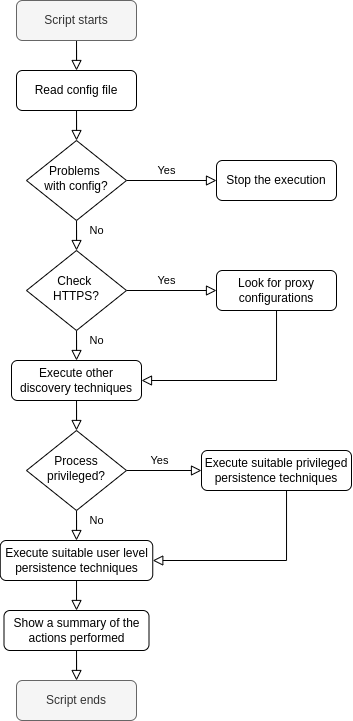
\includegraphics[height=17cm]{img/scriptFlowchart}
	\caption{Flow of the program in a behaviour diagram.}
	\label{img:programFlow}
\end{figure}

\pagebreak
\paragraph{Code sections} 
After the main functionalities of the tool were determined, it was important to segment the code into different parts to organize it, to be able to extend and maintain it effortlessly. 

Using the design and the program flow described above, the code was divided into the following parts:

\begin{itemize}
\item \textbf{Initialization (or Init)}: this part contains all the packages imports, sets default values for variables, and loads the configuration file, which overwrites the default values.

\item \textbf{Discovery functions}: these functions provide the necessary information to later decide which techniques should be applied. They are the ones that: 	
\begin{itemize}
\item Check if a proxy is configured.
\item Try to access the Internet using the protocols HTTPS, DNS, and ICMP, if necessary.
\item Check both the user and the process privileges.
\end{itemize}

Their names are similar in both scripts, but adapted to each programming language code style like \texttt{Check-HTTPS} (PowerShell) and \texttt{check\_https} (Python).

\item \textbf{Persistence techniques}: this part consists of several functions prepared to be deployed according to the operating system tools, like Scheduled Tasks, Startup Folders or the Registry for Windows, and the cronjob or systemd services for Linux. 

\item \textbf{Backdoor mechanisms}: these functions have different goals: some of them perform a reverse connection\footnotemark with a server (defined in the configuration file), and others just change configuration settings in the system, to be able to reach it later. To perform these mechanisms, either pre-installed tools (like RDP or SSH) or external tools can be used. 

\item \textbf{Main function}: this last section contains all the necessary logic to call the most suitable functions on each execution, following the flow described before.
\end{itemize}

The developed code contains several comments, some of them used to divide each one of these sections.  An example of the base file with all the different sections can be seen in Annex \ref{sec:toolCode}.

\footnotetext{ A reverse connection is a communication between a compromised device and an adversary server, started by the first. They are widely used because firewalls tend to restrict connections initiated by external servers.}

\pagebreak
\paragraph{Configuration file}

Since one of the goals of this tool was to be easily adaptable to the needs of its users, and given the amount of different configurable data, an external configuration file has been created to simplify the process of loading different configurations.

This configuration file uses dictionaries in JSON format, because it is widespread and easy to both understand at a glance, and parse in the actual script.

As there are differences between the different operating systems, this file has two types of parameters: common ones and operating system specifics. Nevertheless, the configuration file is divided into different categories, which are common for both scripts. Some of the most important parameters are those described in the table \ref{tab:configFile}.\\

\begin{table}[!htb]
\centering
{\setlength{\tabcolsep}{1em}
  \begin{tabular}{@{\extracolsep{\fill}}| c | c | c | c |}
  \hline \multicolumn{1}{|c|}{\textbf{Type}} & \textbf{Category} & \textbf{Example parameters} & \textbf{Description}\\ \hline \hline 
   \multirow{9}{*}{Shared} & Discovery techniques &  \begin{tabular}{@{}c@{}}- pingTestIP\\ - httpsTestUrl\\ - proxy \end{tabular} & \begin{tabular}{@{}c@{}}Needed to perform\\ discovery tactics\end{tabular}  
  \\ \cline{2-4} & Payload & \begin{tabular}{@{}c@{}} - name\\ - path\\ - URL\\ - pathToSave  \end{tabular} &  \begin{tabular}{@{}c@{}} Data about the file \\ that is going to be \\used to persist \end{tabular}
  \\ \cline{2-4} & Preferences & \begin{tabular}{@{}c@{}}- excludedTechniques\\ - includedTechniques\\ - excludedProtocols\\ - forceProtocols \end{tabular} &  \begin{tabular}{@{}c@{}} To specify which\\techniques are going\\to be executed \end{tabular}
    \\ \hline 	
  \multirow{4}{*}{System specific} & Persistence techniques & \begin{tabular}{@{}c@{}}- cronjobTime\\ - registryKey \end{tabular} & \begin{tabular}{@{}c@{}} Needed to deploy some\\kind of persistence\end{tabular}
  \\ \cline{2-4} & Backdoor techniques & \begin{tabular}{@{}c@{}}- serverIPURL\\ - HTTPSCommand\\ - SSHAuthKey \end{tabular} & \begin{tabular}{@{}c@{}} Needed to deploy some\\kind of backdoors\end{tabular}  
    \\ \hline 
  \end{tabular}}
  \caption{Examples of parameters of the file "\textit{config.json}"} \vspace{3pt}
  \label{tab:configFile}
\end{table}

% Esto lo puedo meter en un readme del config.json
%\begin{itemize}
%\item Shared parameters
%\begin{itemize}
%\item Discovery techniques
%\item Payload settings
%\begin{itemize}
%\item path: to use already downloaded payloads for the deployment.
%\item URL: to download it from the Internet.
%\item pathToSave: if set, a function saves the payload in the specified path.
%\item serverURL: the IP or URL of an external server, for \texttt{SSH} and \texttt{netcat} techniques.
%\item serverPort: the open port of an external server, for \texttt{SSH} and \texttt{netcat} techniques.
%\item HTTPSBack: for external tools, the exact command to execute an HTTPS backdoor.
%\item DNSBack: for external tools, the exact command to execute a DNS backdoor.
%\item ICMPBack: for external tools, the exact command to execute an ICMP backdoor.
%\end{itemize}
%\item Preferences
%\begin{itemize}
%\item excludedTechniques/includedTechniques: to prevent or allow only the execution of certain techniques. 
%\item excludedProtocols/forceProtocols: to prevent or force the checking of certain protocols.
%\end{itemize}
%\end{itemize}
%\item Specific parameters
%\begin{itemize}
%\item Persistence techniques
%\item Backdoor techniques
%\end{itemize}
%\end{itemize}

%There are more configurable parameters, but they are not as relevant as the ones already listed.

An example of the JSON file with the different configuration parameters can be found in Annex \ref{sec:toolCode}.

\pagebreak
To restrict or force the execution of one or several techniques or protocols, there are some keywords, unique for each operating system, that can be used in the "Preferences" parameter to better control the execution flow of the script. These keywords are defined in each script and are available in the "README" file.

Also, some techniques are only executed if their associated configuration setting has a value, like the "downloadFile" function, which is used to download the payload from the Internet, and is executed when the parameter "Payload URL" is not null. Therefore, all these different settings condition the execution of techniques by the entered values; even though, as there are some default values set in the script, not all parameters are needed to run the script.

Another example of this behaviour is the "HTTPSCommand" parameter: the tool would neither search for proxy settings nor check if an HTTPS connection is available if no persistence is planned to be deployed using this protocol. 


